%%%%%%%%%%%%%%%%%%%%%%%%%%%%%%%%%%%%%%%
%  Modèle LaTeX pour les documents TB
%
%  Par Charles Duchêne, IG JI
%  Mai 2013
%
%  Toutes les images doivent se trouver
%  dans un sous-dossier pictures
%
%%%%%%%%%%%%%%%%%%%%%%%%%%%%%%%%%%%%%%%

\documentclass[12pt,a4paper]{article}
\usepackage[utf8]{inputenc} 
\usepackage[T1]{fontenc}
\usepackage[pdftex]{hyperref}	
\usepackage{amsmath}
\usepackage{amsfonts}
\usepackage[english,francais]{babel}
\usepackage{telecom}	
\usepackage{aeguill}
\usepackage{times}
\usepackage{listingsutf8}
\usepackage{makeidx}
\usepackage[style=tree,order=word,nonumberlist]{glossaries}
\usepackage{lipsum}
\usepackage{wrapfig}

%%%%%%%%%%
\usepackage{listings} 			% para llistas de codigo

%%%%%%%%%%%%
\makeindex
\makeglossary

%%%%%%%%%%%%%%%%%%%%%%%%%%%%
% Variables pour ce document
%%%%%%%%%%%%%%%%%%%%%%%%%%%%
\author{Lucas PEREIRA ENDRES}
\title{Developpement d'un multiplexeur MPEG2 compatible avec le standard SBTVD de télévision numérique}
%\contributors{}
\version{1.0}
\docdescription{\textbf{Tuteur au Brésil:} \\ Altamiro Amadeu SUSIN \\ \textbf{Évalué par:}\\ Michel JEZEQUEL \\ Sylvie KEROUEDAN\\ \- \\Rapport de Stage de Fin d'Études}
%%%%%%%%%%%%%%%%%%%%%%%%%%%
%%% FICHIER DE CONFIGURATION OPTIONNEL

%%%%%%%% Propriétés pdf %%%%%%%%%%%
\hypersetup{
	bookmarks=true,
	unicode= yes,
	pdftitle={Document témoin du modèle LaTeX pour Télécom Bretagne},
	pdfauthor={Charles Duchêne},
	pdfsubject={},
	pdfkeywords={Télécom, TB, modèle, LaTeX},
	colorlinks=true,
	linkcolor=black,
	citecolor=black,
	filecolor=black,
	urlcolor = black
}

\lstset{
	basicstyle=\ttfamily\small,
	breaklines=true,
	keywordstyle=\bfseries\color{TBbrun},
	inputencoding=utf8/latin1,
}

\lstdefinestyle{stylelatex}{%
	language=tex,
	morekeywords={usepackage,newcommand,begin,renewcommand,section,
	TBannexe,TBsommaire,subsection},
	commentstyle=\itshape\color{TBvert}
}

\lstnewenvironment{latex}{%
	\lstset{style=stylelatex}}{}

\lstnewenvironment{bash}{%
\lstset{
	language=bash,
	basicstyle=\color{white}\ttfamily\small,
	keywordstyle=\color{TBvert}\bfseries,
	backgroundcolor=\color{black},
	morekeywords={sudo, cp, mkdir},
	deletekeywords={local},
}
}{}
 % fichier de configuration optionnel

\lstset{
	basicstyle=\footnotesize\ttfamily,
	%framextopmargin=50pt,
	%frame=lrtb
    language=C,
    frame=single,
    tabsize=2,
    showspaces=false,
    showstringspaces=false,
    keywordstyle=\color{blue},
    %morekeywords={QStringList,QDate,QString,QIODevice},
    commentstyle=\color{CadetBlue},
    %caption={Zistenie, či sme v daný deň, už záznam o rýchlosti uložili},
    breaklines=true
	}

%%%% DÉBUT DOCUMENT
\begin{document}
% ne pas modifier ! imprime la première page du document
\TBfrontcover
\newpage
%%%%%%%%%%%%%%%%%%%%%%%%%%%%
%     CORPS DU DOCUMENT
%%%%%%%%%%%%%%%%%%%%%%%%%%%%
 
\newpage
\section*{Résumé}
La télévision est, parmi les médias de diffusion, le plus important au Brésil. Au début de la dernière décennie, il a été décidé de numériser le système de diffusion de télévision brésilienne. Une action du gouvernement en rejoignant des entreprises et chercheurs de tout le pays a réalisé une étude sur plusieurs sujets de la télévision
numérique. Codage vidéo et audio, ainsi que les sous-systèmes d’interactivité, de multiplexage, de modulation et de transmission sont parmi les aspects étudiés du
système Numérique. Ce qui est ressorti est le SBTVD, le standard de télévision numérique brésilien, qui est basé sur la norme de transmission japonaise, ISDB-T, et
adopte H.264 et HE-AAC comme standards de codage vidéo et audio. Aujourd’hui, la quasi-totalité de l’Amérique du Sud et certains pays africains ont adopté le SBTVD.
L’objectif principal de ce travail est de développer un outil qui crée un flux de transport conforme à la norme brésilienne ABNT NBR15603, à sa fois basée sur la
norme ISO/IEC 13818-1. Pour atteindre cet objectif, une recherche considérable a été réalisée pour comprendre les concepts fondamentaux introduits par ISO/IEC13818-1
et les différences entre cette norme et l’ABNT NBR15603. Certains outils existants génèrent des flux conformes aux normes internationales, mais ne parviennent pas à respecter les spécificités du SBTVD. Une version mise à jour du framework FFmpeg est donc proposée, qui comprend maintenant les structures de données obligatoires
de le SBTVD dans le flux de transport.

\newpage
\section*{Abstract}
Television is the most important broadcast media in Brazil. At the beginning of the last decade, it was decided to digitize the Brazilian TV broadcast system. A government action joining researchers of all around the country carried out a study on several topics of Digital TV. Video and audio coding, along with interactivity and multiplexing, modulation and transmission subsystems are among the studied aspects of the DTV System. What came out is the SBTVD, the Brazilian DTV standard, which is based on the Japanese ISDB-T transmission standard, and adopts H.264 and HE-AAC as video and audio coding standards. Nowadays, almost all South American and some African countries adopted the SBTVD. The main objective of this work is to develop a tool that creates a Transport Stream compliant to the Brazilian standard ABNT NBR15603 which is based on the ISO/IEC 13818-1 standard. To achieve this objective, considerable research was carried out to understand the fundamental concepts introduced by ISO/IEC13818-1 and the differences between this standard and the ABNT NBR15603. Some existing tools generate streams compliant to the international standards but fail to obey the Brazilian specificities. An updated version of the FFmpeg framework is therefore proposed which now includes the mandatory structures of SBTVD in the Transport Stream.


%% Affichage des listes et tables.
\newpage
\listoffigures  % commenter pour ne pas avoir la liste des figures
\listoftables   % commenter pour ne pas avoir la liste des tables
\newpage
\TBsommaire

\section*{Avertissement / Disclaimer}

\-\newline
Ce travail a été élaboré sur la base de la collection de logiciels FFmpeg \cite{ffmpeg} et est soumis à la licence LGPL v2.1 \cite{gplv2}. La partie modifiée du code de FFmpeg est dans la bibliothèque «avformat», qui est le droit d'auteur (C) 2003 de Fabrice Bellard. L'encodeur H.264 utilisé pour créer les échantillons de flux vidéo de ce travail est soumis à la licence GPL et est Copyright (C) 2005 de Rullgard Mans (mans@mansr.com). L'auteur est prêt à aider quiconque est intéressé à obtenir plus d'informations sur les conditions d'octroi de licences.

\-\newline
This work was developed based on the FFmpeg\cite{ffmpeg} framework and is subject to the LGPL v2.1 Licence \cite{gplv2}. The modified part of FFMpeg code is within the 'avformat' library, which is Copyright (C) 2003 of Fabrice Bellard. The H.264 encoder used to create the sample video streams in this work is licenced under the GPL v2 Licence and is Copyright (C) 2005 of Mans Rullgard ( mans@mansr.com). The author is willing to help whomever is interested in obtaining further information on licencing conditions.

\-\newline
\begin{minipage}{\linewidth}
\begin{lstlisting}[]
FFmpeg is free software; you can redistribute it and/or modify it under
the terms of the GNU Lesser General Public License as published by the
Free Software Foundation; either version 2.1 of the License,
or(at your option) any later version.

FFmpeg is distributed in the hope that it will be useful, but WITHOUT
ANY WARRANTY; without even the implied warranty of
MERCHANTABILITY or FITNESS FOR A PARTICULAR PURPOSE.
See the GNU Lesser General Public License for more details.

You should receive a copy of the GNU Lesser General Public License
along with FFmpeg; if not, write to the Free Software Foundation, Inc.,
51 Franklin Street, Fifth Floor, Boston, MA 02110-1301 USA.
\end{lstlisting}
\end{minipage}

\-\newline
Les codes sources pour cette modification du code de FFmpeg est disponible en Internet sous le système de contrôle de versions Git, à l'addresse suivante:

\-\newline
The source code for this modification is publicly available in the Internet under Git version control system, and may be accessed via the following link:
\begin{verbatim}
https://github.com/nasall2/TCC_ffmpeg
\end{verbatim}

%%%%%% INICIO DO TEXTO PROPRIAMENTE DITO

\newpage
\section{Introduction}

Historiquement, la télévision est présente dans les maisons de la plupart des citoyens brésiliens et il est la principale source de divertissement et d'information à la population. Au cours des 10 dernières années, les nouveaux médias numériques tels que les téléphones portables et d'ordinateurs sont en cours d'adoption par la population de différentes classes sociales. Un récent rapport de \cite{pnad2011} dit que, en 2011, 69 \% de la population avait une ligne de téléphone mobile. Bien que significative, la participation de ce média reste largement inférieur à celle de la télévision, dont la zone de couverture atteint 100 \% du territoire via satellite \cite{StarOne}, et environ 98 \% de la population par voie terrestre \cite{globo}. La télévision est donc la principale voie de communication à la disposition du grand public au Brésil.

Bien qu'il dispose d'une couverture inégalée à d'autres technologies, la télévision a été traditionnellement utilisé pour la communication unidirectionnelle. Il n'est pas possible, en utilisant le système de transmission de la télévision analogique, rendre au spectateur de l'intéractivité avec le contenu soumis par la chaîne de télévision. Par rapport à \textit{Internet}, par exemple, la télévision est en désavantage dans cet aspect. Il est possible, toutefois, de prévoir la programmation interactive si il ya un moyen de renvoyer des données au radiodiffuseur. Avec l'interactivité, il peut être présenté des options de programmation à l'utilisateur, et à partir du choix de l'utilisateur, le téléviseur affiche le contenu choisi. Ainsi, on pourrait combiner l'interactivité de \textit{Internet} à la couverture de la télévision et ainsi favoriser l'inclusion sociale des zones reculées sans accès aux infrastructures de liaisons de données à grande vitesse, disponibles dans les grandes villes. Cette technologie n'est pas possible avec l'infrastructure de télévision analogique actuelle: il est impossible de transmettre viaun seul canal analogique plusieurs vidéos et audio simultanément .

Comme solution à cette difficulté, la norme ISO/IEC a développé le système de transmission numérique décrit par la norme ISO/IEC13818-1, commercialement connu sous l'acronyme qui désigne le comité formé pour la rédiger, MPEG2, ou aussi connu comme la recommandation ITU-T H .222. La spécification décrit les normes de codage et transmission de vidéo ,audio et des données du système. Une caractéristique clé pour les applications de télévision, c'est qu'il est possible de diffuser des programmes audiovisuels multiples simultanément, permettant ainsi à l'utilisateur de sélectionner les informations qu'il souhaite recevoir parmi plusieurs services envoyés par un seul diffuseur, dans le même canal physique.

Au Brésil, depuis 1994, les entreprises privées et le gouvernement ont financé de la recherche et des tests techniques à fin de comparer la performance de trois systèmes de télévision numérique qui ont été connus pour être efficaces dans leurs pays d'origine à l'époque: ATSC \cite{ATSC}, développé aux Etats-Unis; DVB-T \cite{DVB}, développé par un consortium d'entreprises pour une utilisation dans les pays européens; et ISDB, développé au Japon par ARIB \cite{ARIB}. Les trois systèmes ont des similitudes et des différences en ce qui concerne l'encodage vidéo et audio: pour exemple, la DVB et ISDB utilisent l'infrastructure de transport de la norme MPEG2, mais diffèrent dans les schémas de modulation. Après les évaluations, il a été déterminé que le système le plus performant pour le territoire brésilien serait basée sur l'ISDB japonais avec quelques modifications, comme indiqué dans le decret presidentiel de création du système\cite{decreto8061}.

Les différences entre l'original et ISDB la norme modifiée utilisée au Brésil concernent principalement l'encodage vidéo et plate-forme d'interactivité. Afin de promouvoir le développement de l'industrie nationale, le gouvernement a décidé d'adopter une plate-forme open source interactive, élaborée avec Ginga, une technologie développée principalement par des chercheurs brésiliens \cite{PUCRJ}. Grâce à cet outil, le diffuseur peut, par exemple, fournir des informations utiles à la population à faible revenu qui n'ont pas accès à \textit{Internet}, comme par exemple une application proposée par une banque brésilienne en 2010 \cite{caixa}. Une autre application est un projet récemment mis au point par la entreprise publique de comunication (EBC), appelé "Brasil 4D" \cite{consultas}. Les utilisateurs peuvent prendre rendez-vous avec les médecins ou planifier des réunions pour résoudre les problèmes de sécurité sociale, ou encore consulter les offres d'emploi en temps réel, tout cela à travers la télécommande du téléviseur. Cependant, la similitude du système brésilien à la norme internationale et le fait que les interfaces interactives ne sera pas obligatoire avant 2015 a conduit à un manque d'intérêt de nombreux diffuseurs dans le développement d'applications, de sorte qu'à l'heure actuelle très peu a été investi dans la création de télévision numérique interactive sur le territoire brésilien.

Un système de télévision numérique est composé essentiellement par le groupe d'équipements présentés dans la \autoref{fig:diagrama_blocos_tvd}. Au début de l'écoulement du signal, il y a des éléments de capture de vidéo et audio, tels que des caméras et des micros, et le signal brut peut être analogique ou numérique en fonction de la technologie de capture utilisé. Une fois capturés, la vidéo et l'audio sont compressées et codées par des codeurs correspondants. Le résultat des codeurs sont bitstreams standardisés appelés flux élémentaires. Une fois que les flux élémentaires quittent les codeurs, ils entrent dans le multiplexeur, où tous les flux élémentaires sont mis en paquets et intégrés dans un seul flux, ce qui est l'objectif principal de la couche système de MPEG2. Ce qui suit est un processus clé pour la robustesse du système: le flux est protégé par l'emploi de codes de correction d'erreur pour résister au bruit du canal à trajets multiples entre le diffuseur et le récepteur. Enfin, une modulation numérique est appliqué et le flux modulé est envoyé à l'antenne.

 \begin{figure}[!h]
\centering
\caption{Schéma simplifié des flux de signal de la télévision numérique.}
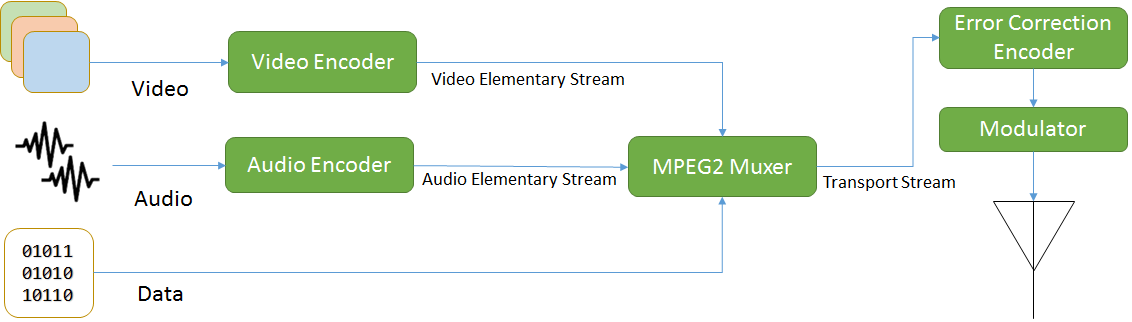
\includegraphics[width=1\linewidth]{pictures/diagrama_blocos_tvd.png}
\label{fig:diagrama_blocos_tvd}
\end{figure}
 
La principale différence entre les systèmes de télédiffusion analogique et numérique, au niveau de la modulation, est que, dans la télévision analogique le multiplexage est dans le domaine fréquence, le signal vidéo est envoyé dans une bande de fréquence comprise dans la bande passante de canal et le signal audio dans une autre bande de fréquence. Dans la technologie numérique, le multiplexage se passe dans le domaine temporel: la sortie du multiplexeur a un débit constant, et pour les fractions de seconde seulement un paquet d'une des sources de média est envoyé à l'émetteur. De l'autre côté du canal, le récepteur est conçu de manière à ce que, après passage de la couche de correction d'erreur, un \textit{démultiplexeur} prend le flux composé et le sépare de nouveau dans les flux binaires élémentaires. Ils sont ensuite envoyés aux décodeurs et aux dispositifs de sortie audiovisuels.

Il serait certainement troublant pour le spectateur à regarder les contenus vidéo ou audio en différé, ainsi un défi de ce schéma de multiplexage est de synchroniser la reproduction de tous les flux de média Pour ce faire, des labels d'horodatage de présentation sont ajoutés périodiquement dans les flux afin qu'ils puissent être reproduits au même temps.

Le Loi Presidentiel 8061 \cite{decreto8061} du 29 juillet 2013 établit le chronogramme d'arrêts des transmissions analogiques. Jusqu'au 31 décembre 2018, tous les émetteurs analogiques seront désactivés et les canaux doivent être libérées. Les droits d'éxploitation des radiofréquences seront ensuite remis au gouvernement, qui prévoit d'utiliser la bande de 700 MHz pour le service de téléphonie mobile 4G LTE.

L'objectif de ce projet est de développer un outil simple, mais flexible, pour gérer la couche des systèmes de la norme SBTVD. Fondamentalement, en utilisant cet outil on est capable de produire un fichier binaire compatible avec le système SBTVD, contenant un flux de transport qui peut être utilisé pour diffuser de la vidéo enregistrée et les flux audio dans des récepteurs appropriés. Beaucoup de solutions commerciales pour cet objectif sont disponibles sur le marché, de sorte que la cible ici n'était pas de développer un produit de consommation, mais plutôt quelque chose de plus académique, éducatif, où la plupart des configurations peuvent être modifiées selon les besoins. Le client interne principal à l'université (UFRGS) est le projet du \textit{set-top-box} SBTVD, qui développe un boîtier décodeur du système numérique dans une architecture \textit{System on Chip} sur FPGA. Pour exécuter les tests de l'ensemble du système, les flux de transport avec différentes configurations de multiplexage doivent être diffusées à fin de tester le décodeur sur des cas spécifiques.

Le flux de travail du projet était le suivant. La première étape a consisté à étudier la norme ABNT NBR15603, ainsi que les références à la norme ISO/IEC 13818 et à la norme ARIB STD-B10. Dans cette partie, l'objectif était de comprendre comment la couche Système devrait travailler, identifier les composants du multiplexeur qui étaient obligatoires et facultatifs. En discutant le projet aux premières semaines, il a été décidé d'évaluer la possibilité de développer l'outil à partir de zéro. C'était avant que la première étape avait été accomplie, parce que d'autres personnes dans le laboratoire avaient déjà fait des recherches et avaient conclu que outils gratuits disponibles ne pouvaient pas gérer les flux selon le standard SBTVD. Au cours de recherches menées par l'auteur sur l'Internet des outils intéressants ont été identifiés. Ainsi, au lieu de développer à partir de zéro l'outil, il semblait alors plus raisonnable de profiter d'un \textit{framework} existant.

Une fois qu'il étant décidé que un outil existant serait modifié, la troisième étape a consisté d'ajouter les fonctionnalités manquantes afin de rendre l'outil compatible avec le SBTVD. Finalement, les caractéristiques ont été testés sur diférents récepteurs. L'objectif pratique du projet est de fournir un outil qui crée des flux de transport avec trois caractéristiques principales: présentation audiovisuelle synchrone, conformité à la norme SBTVD et possibilité d'envoi de multiples services. Finalement si des structures obligatoires sont qu'à titre d'information et son absence ne bloque pas le système, ils pourraient être laissés au développement futur.

TODO Ajouter la structure du laboratoire, le plan de travail, quelques comentaires à propos du nombre d'heures,

%\subsection{}
%\subsubsection{}


% ANNEXES
\appendix
%\index{Annexe}
\TBannexe{Blah blah}
\section{Test}
\newpage
\TBannexe{Buh Buh}
\section{123}
\subsection{222}
\subsection{444}

\newpage
% INDEX, RÉFÉRENCES et GLOSSAIRE
 %\TBindex
 \TBbiblio{plain-fr}{includes/biblio}
 \TBglossary

% ne pas modifier ! imprime la dernière page du document
\TBcoverpage
\end{document}
